\documentclass[a4paper, 11pt]{exam}
\usepackage[utf8]{inputenc}
\usepackage{hyperref}
\usepackage{graphicx}
\usepackage{subfig}
\usepackage[export]{adjustbox}

\title{Clustering en Weka}
\author{Laura Rodríguez Navas \\ rodrigueznavas@posgrado.uimp.es}
\date{\today}

\pagestyle{plain}

\begin{document}
	
\maketitle

\renewcommand{\figurename}{Figura}
\renewcommand{\tablename}{Tabla}


En esta práctica vamos a realizar un estudio acerca de los datos de Iris. Esta BD se distribuye junto a la herramienta \href{https://www.cs.waikato.ac.nz/ml/weka/}{Weka}. Toda la información sobre esta BD se puede encontrar en el siguiente enlace: \url{https://archive.ics.uci.edu/ml/datasets/Iris}. La BD contiene 4 variables descriptivas y una variable clase. Dado que no contiene valores perdidos, no deberemos de eliminarlos antes de continuar el análisis. Además, como las variables descriptivas son numéricas no deberemos de transformarlas.

\vspace{3mm}
Debido a que los algoritmos de clustering se basan en el cómputo de valores de distancias entre los grupos, es ventajoso tener todas las variables en la misma escala para el cálculo de las distancias entre grupos. Así que, vamos a convertir todas las variables descriptivas a una misma escala. Para ello, vamos a utilizar un filtro de atributo de tipo no supervisado llamado \textit{Standardize} (ver Figura \ref{Figura_1}), y vamos a ignorar la variable clase durante el proceso.

\vspace{5mm}
\begin{figure}[h]
	\centering
	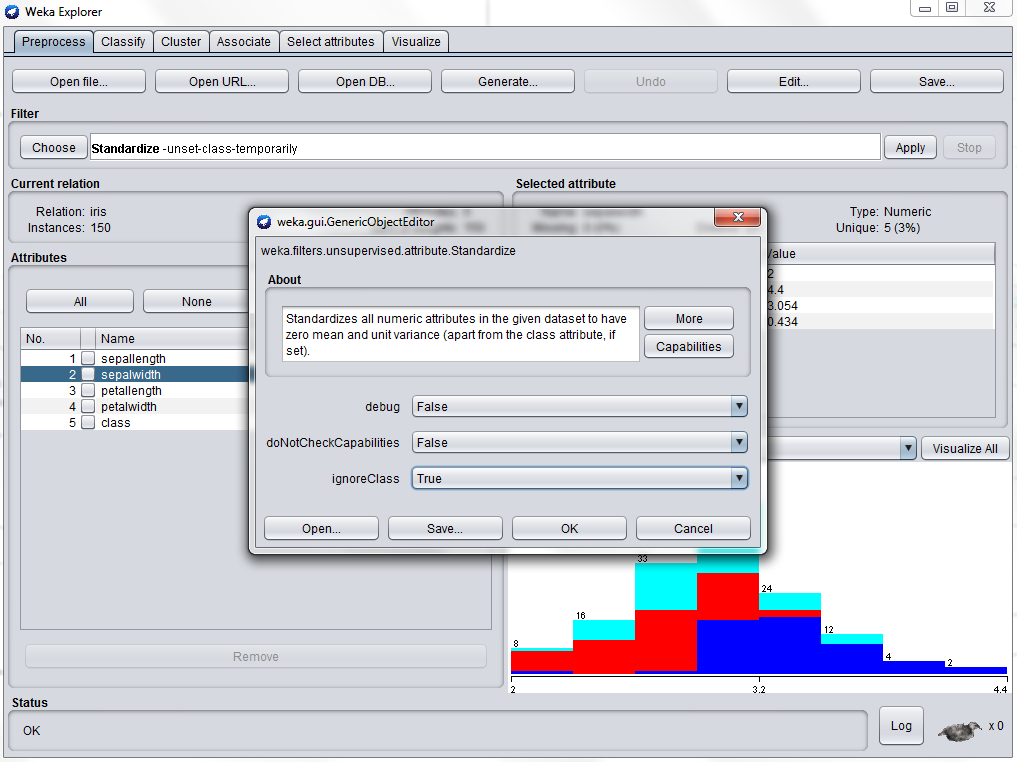
\includegraphics[width=0.6\textwidth]{iris_scaled.png}
	\caption{Filtro \textit{Standardize}.}
	\label{Figura_1}
\end{figure}

La variable clase no se debe tener en cuenta a la hora de realizar el clustering, ya que estamos haciendo un aprendizaje no supervisado, y por tanto la vamos a eliminar. Para ello, vamos a utilizar un filtro de atributo no supervisado llamado \textit{Remove} (ver Figura \ref{Figura_2}).

\begin{figure}[h]
	\centering
	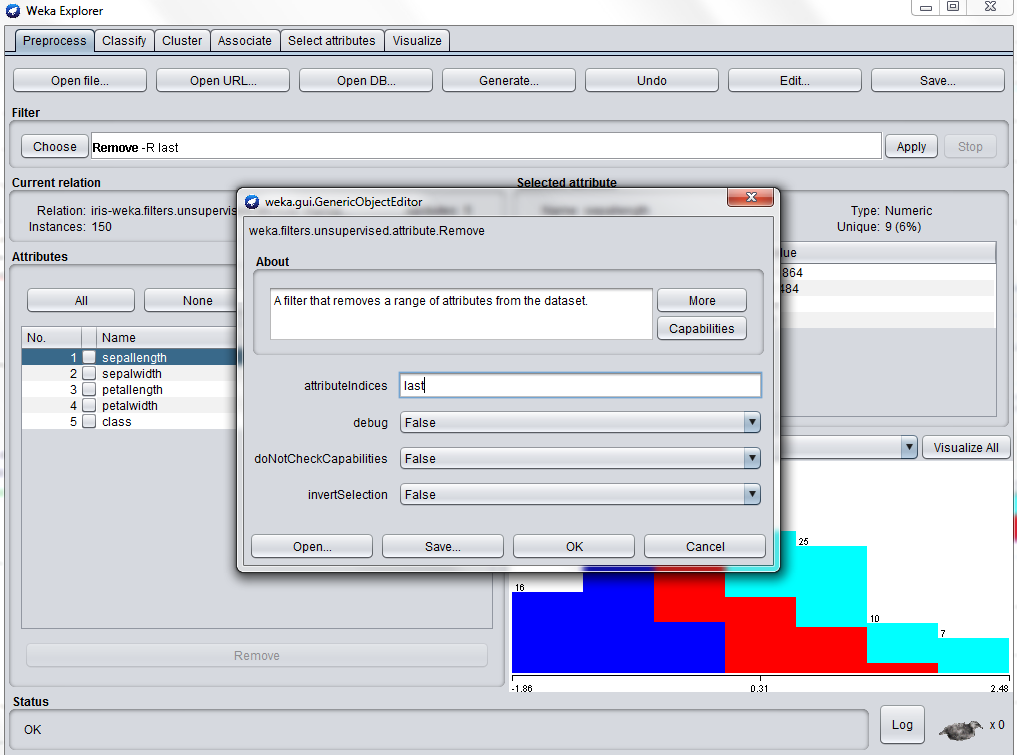
\includegraphics[width=0.6\textwidth]{iris_sin_class.png}
	\caption{Filtro \textit{Remove}.}
	\label{Figura_2}
\end{figure}

\newpage
\begin{questions}
	
% Pregunta 1
{\question Ejecuta el algoritmo SimpleKMeans usando la herramienta Weka con las distancias Euclídea y Manhattan.}

\begin{figure}[h]
	\centering
	\subfloat[con distancia Euclídea.]{{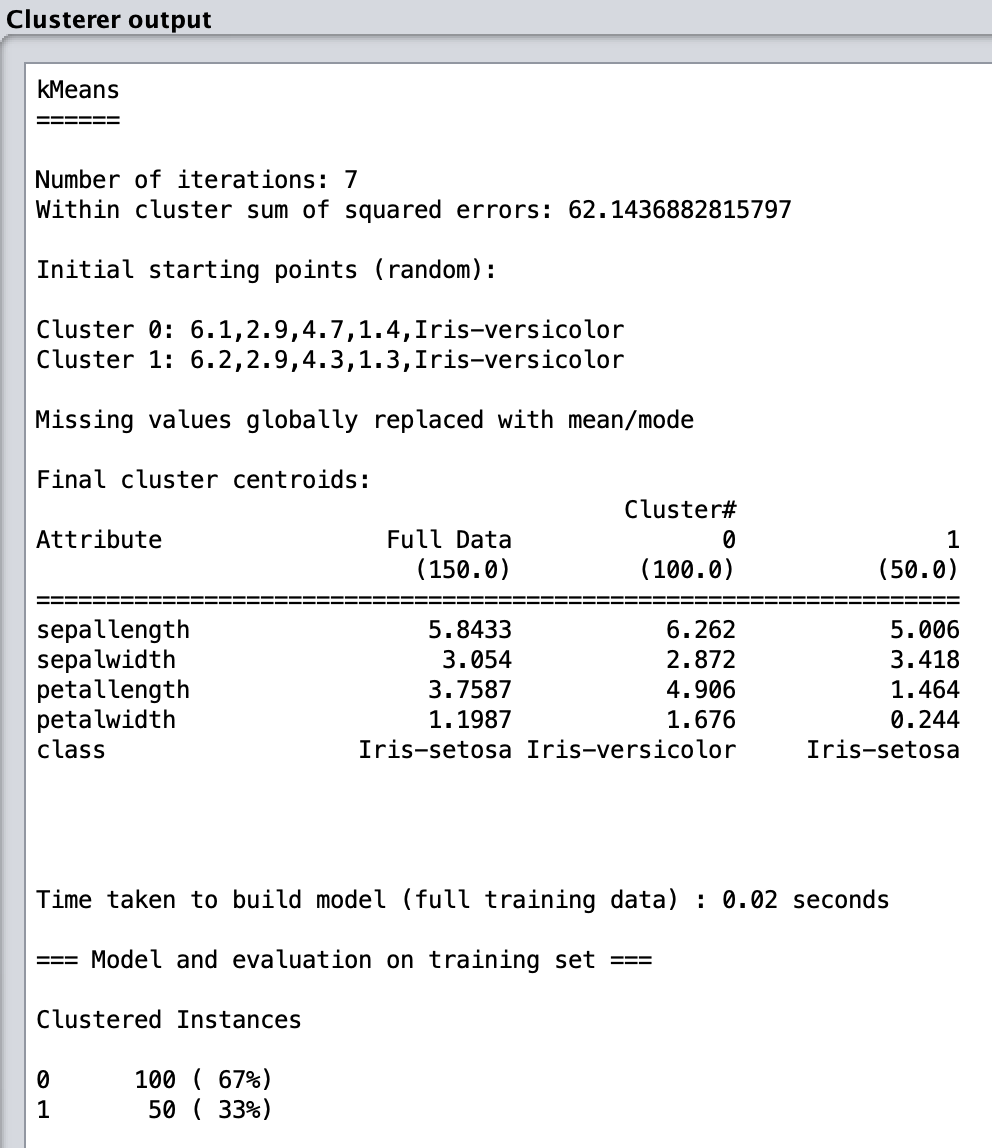
\includegraphics[width=6cm]{kmeans_euclidea.png} }}
	\qquad
	\subfloat[con distancia Manhattan.]{{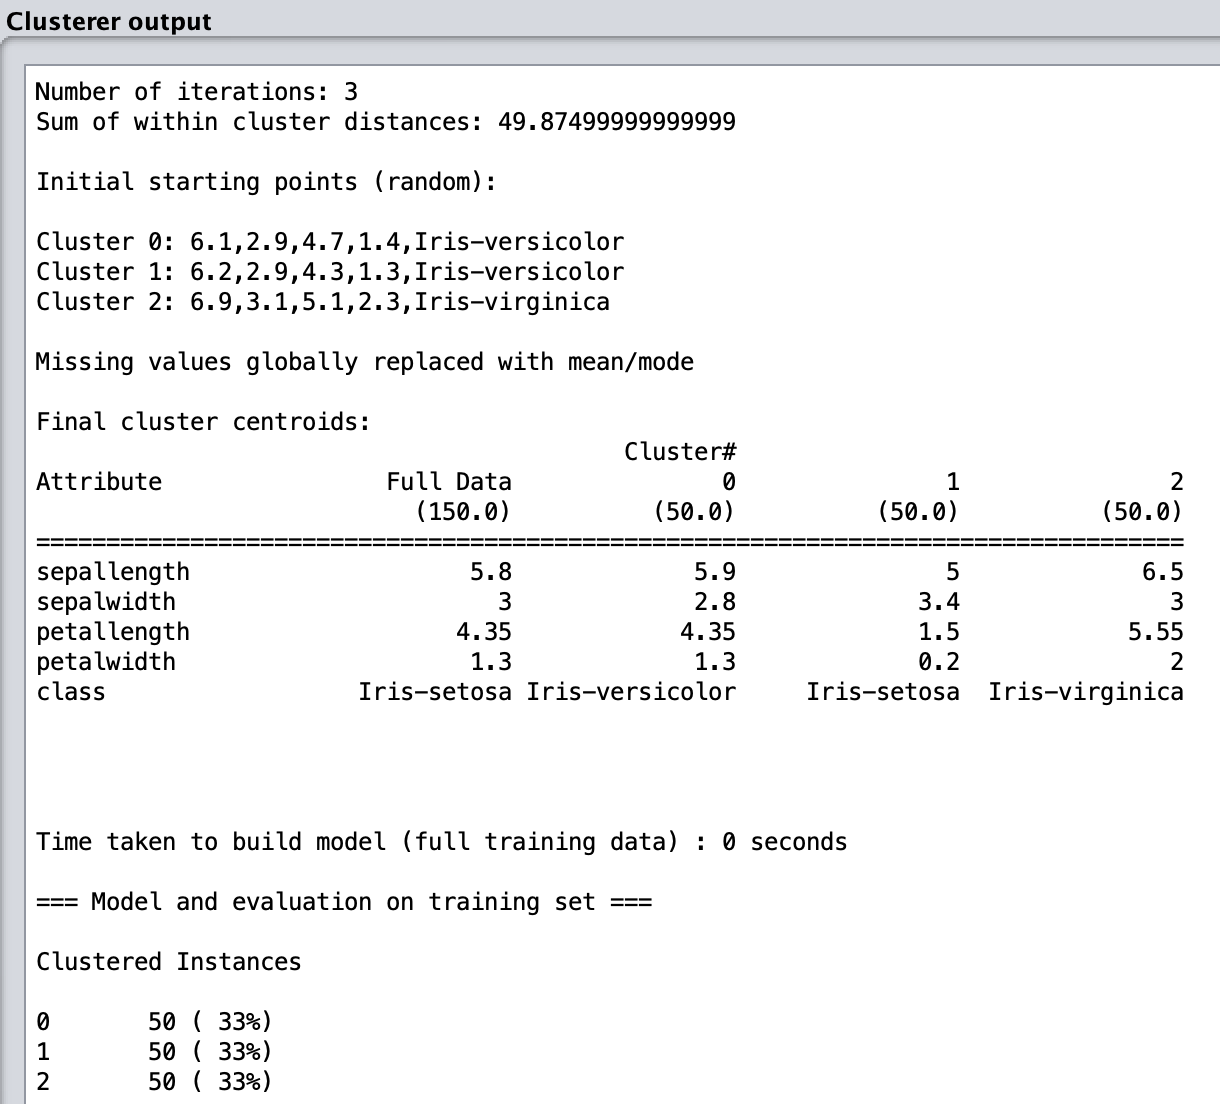
\includegraphics[width=6cm]{kmeans_manhattan.png} }}
	\caption{SimpleKMeans.}
	\label{Figura_3}
\end{figure}

Nota: Como la variable de clase puede tomar 3 valores diferentes, hemos elegido que el valor de \textit{k} sea igual a 3. 

Si nos fijamos en el valor de SSE, vemos que el primer clustering con distancia Euclídea ha funcionado mejor, ya que el valor de SSE es pequeño (6.998). En cambio, el clustering con distancia Manhattan no ha funcionado muy bien, ya que el valor de SSE es muy alto (47.779). Para mejorar el segundo clustering, tendríamos que augmentar el valor de \textit{k}.

\begin{parts}
	
\newpage
\part ¿Cuántas instancias contiene cada grupo?

En la Figura \ref{Figura_3} podemos ver las instancias que contienen cada grupo (0, 1 y 2), que se resumen en la siguiente Tabla \ref{Tabla_1}.

\begin{table}[h] 
	\begin{center}
		\begin{tabular}{|c|c|c|c|}
			\hline
			Distancia & Grupo 0 & Grupo 1 & Grupo 2 \\ \hline
			Euclídea & 61 & 50 & 39 \\ \hline
			Manhattan & 62 & 50 & 38 \\ \hline
		\end{tabular}
	\end{center}
	\caption{Instancias de cada grupo en SimpleKMeans.}
	\label{Tabla_1}
\end{table}

\part ¿Cuáles son los centroides?

Si nos volvemos a fijar en la figura \ref{Figura_3}, podemos observar los centroides de cada ejecución de SimpleKMeans, que se muestran más detalladamente en la siguiente figura.

\begin{figure}[h]
	\centering
	\subfloat[con distancia Euclídea.]{{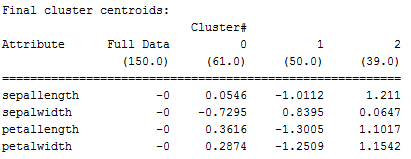
\includegraphics[width=7cm]{kmeans_euclidea_centroides.png} }}
	\qquad
	\subfloat[con distancia Manhattan.]{{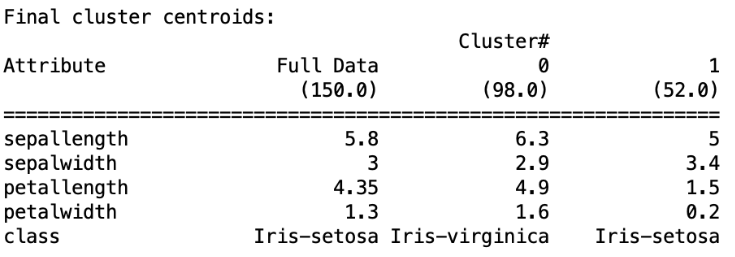
\includegraphics[width=7cm]{kmeans_manhattan_centroides.png} }}
	\caption{Centroides en SimpleKMeans.}
	\label{Figura_4}
\end{figure}

\part Analiza los centroides. ¿Hay algo destacable en esos centroides? ¿Están los centroides separados en el espacio? ¿Tienen componentes similares?

En general, vemos que hay bastante cohesión entre los centroides, eso quiere decir que tienen componentes muy similares. Por ejemplo, el grupo 0 presenta mucha cohesión. También vemos que existe mucha separación entre los centroides. A continuación, podemos observar visualmente la separación entre los centroides (ver Figura \ref{Figura_5}).

\begin{figure}[h]
	\centering
	\subfloat[con distancia Euclídea.]{{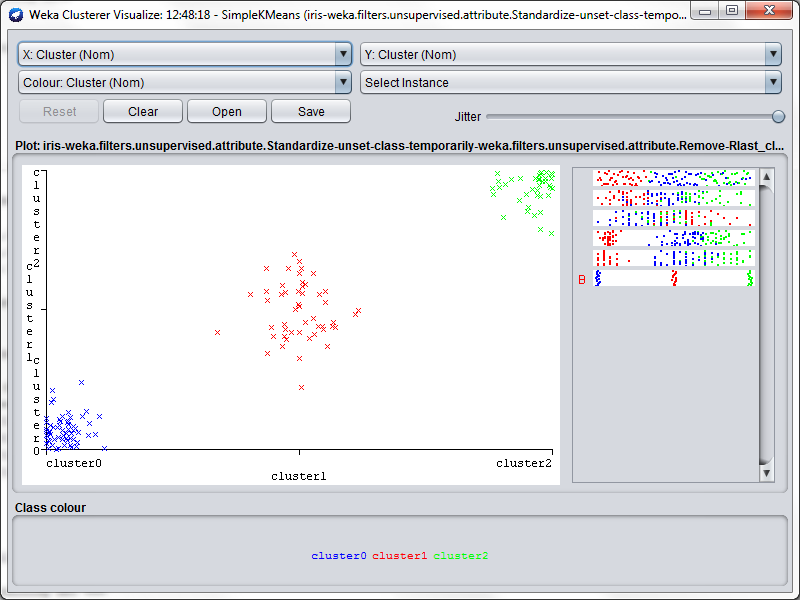
\includegraphics[width=7cm]{kmeans_euclidea_centroides_graph.png} }}
	\qquad
	\subfloat[con distancia Manhattan.]{{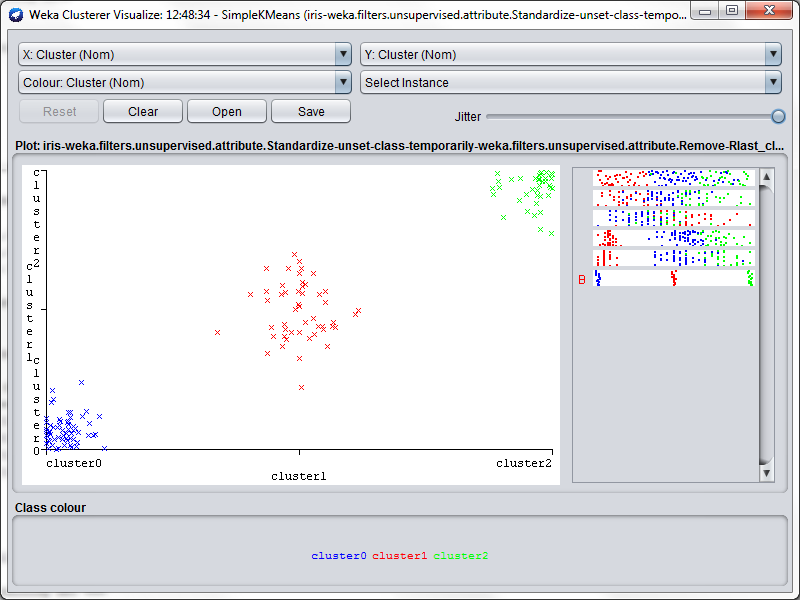
\includegraphics[width=7cm]{kmeans_manhattan_centroides_graph.png} }}
	\caption{Centroides en SimpleKMeans.}
	\label{Figura_5}
\end{figure}

\end{parts}

% Pregunta 2
{\question Ejecuta el algoritmo HierarchicalClusterer con tipo de enlace completo y métrica de distancia Euclídea, y visualiza las gráficas de los puntos agrupados. ¿Alguna de ellas produce grupos bien diferenciados y con fronteras claras?}

Nota: Compara que el eje X instance\_number y el eje Y vaya variando y muestra cada una de las variables (debes adjuntar las imágenes).

Nota: Volvemos a elegir para la ejecución del algoritmo que el valor de \textit{k} sea igual a 3.

El resultado de la ejecución del algoritmo HierarchicalClusterer se puede observar en la siguiente figura:

\begin{figure}[h]
	\centering
	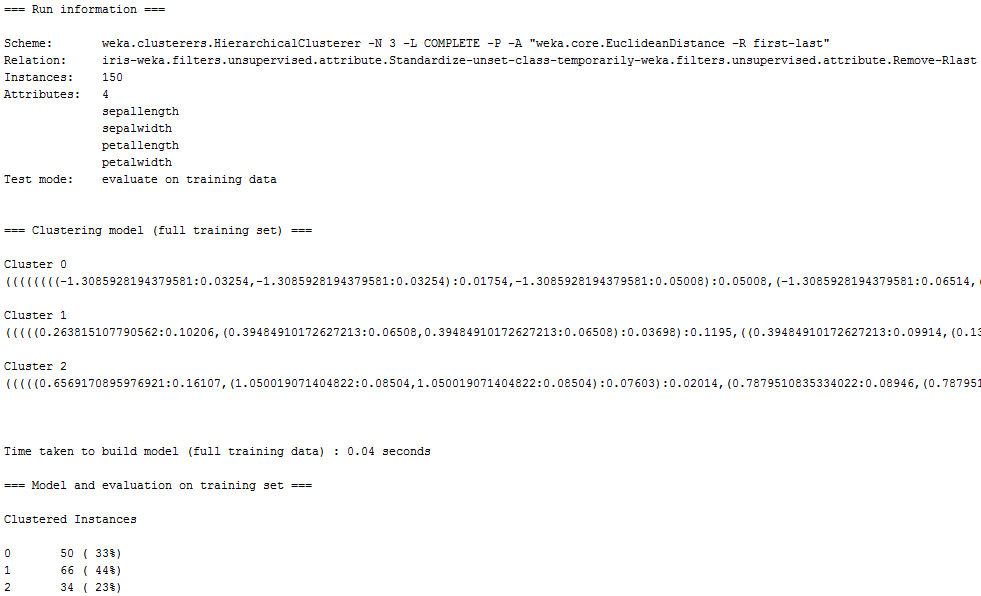
\includegraphics[width=0.8\textwidth]{hc_euclidea.png}
	\caption{HierarchicalClusterer con distancia Euclídea.}
	\label{Figura_6}
\end{figure}

La ejecución del algoritmo HierarchicalClusterer ha formado el grupo 0 con 50 instancias, el grupo 1 con 66 instancias, y el grupo 2 con 34 instancias. Aunque el valor de \textit{k} es el mismo que en la ejecución del algoritmo SimpleKMeans, no se obtiene el mismo resultado (ver Tabla \ref{Tabla_1}).

A continuación se visualizan ls gráficas de los puntos agrupados para cada variable descriptiva del eje Y con el eje X instance\_number.

\begin{itemize}
	\item \textit{sepallength} y \textit{sepalwidth}
	\begin{figure}[h]
		\subfloat[con Y \textit{sepallength}.]{{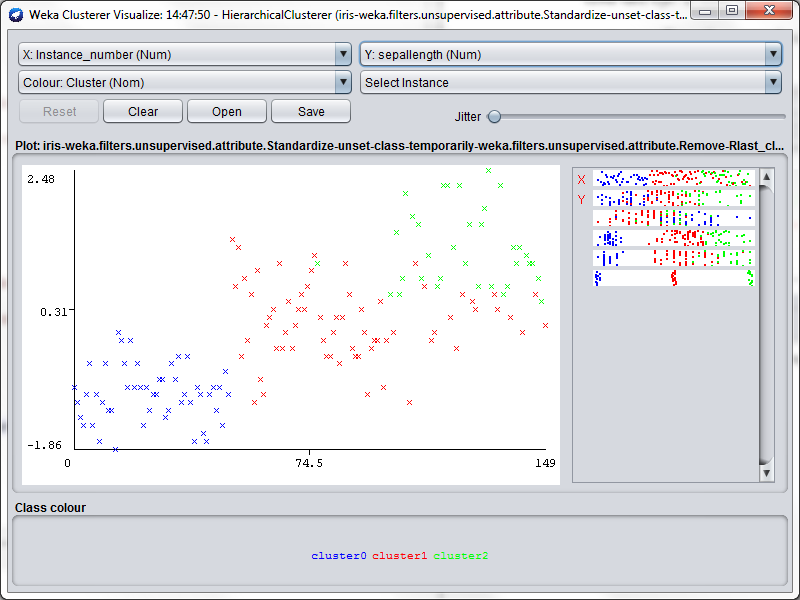
\includegraphics[width=8cm]{hc_sepallength.png} }}
		\qquad
		\subfloat[con Y \textit{sepalwidth}.]{{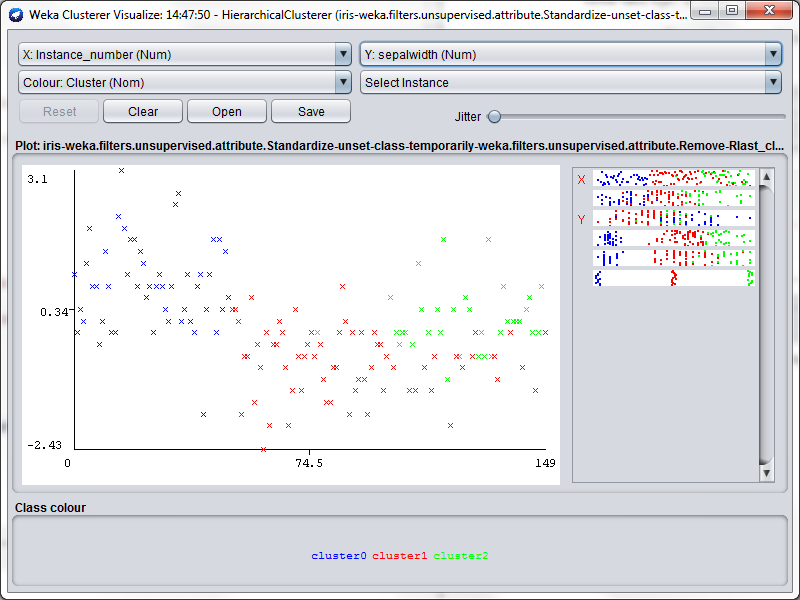
\includegraphics[width=8cm]{hc_sepalwidth.png} }}
		\caption{X instance\_number con \textit{sepallength} y \textit{sepalwidth}.}
		\label{Figura_7}
	\end{figure}
	\newpage
	\item \textit{petallength} y \textit{petalwidth}
	\begin{figure}[h]
		\subfloat[con Y \textit{petallength}.]{{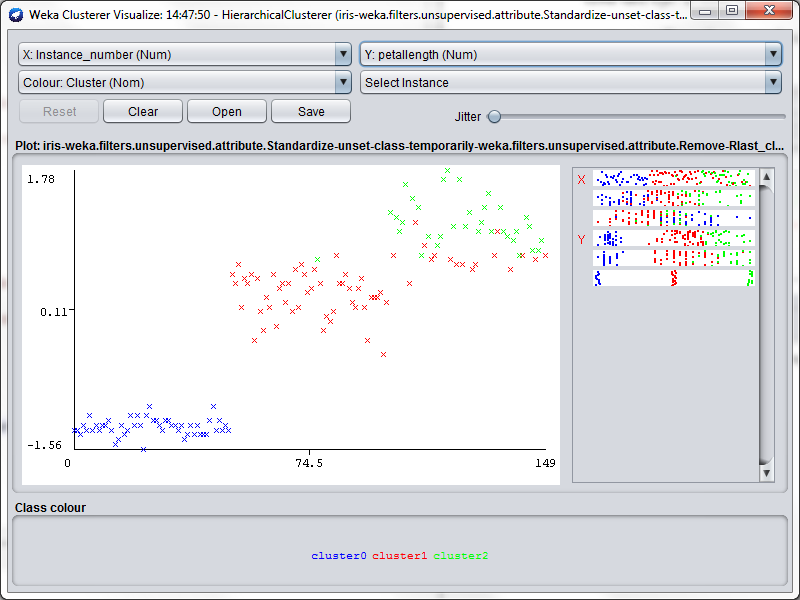
\includegraphics[width=8cm]{hc_petallength.png} }}
		\qquad
		\subfloat[con Y \textit{petalwidth}.]{{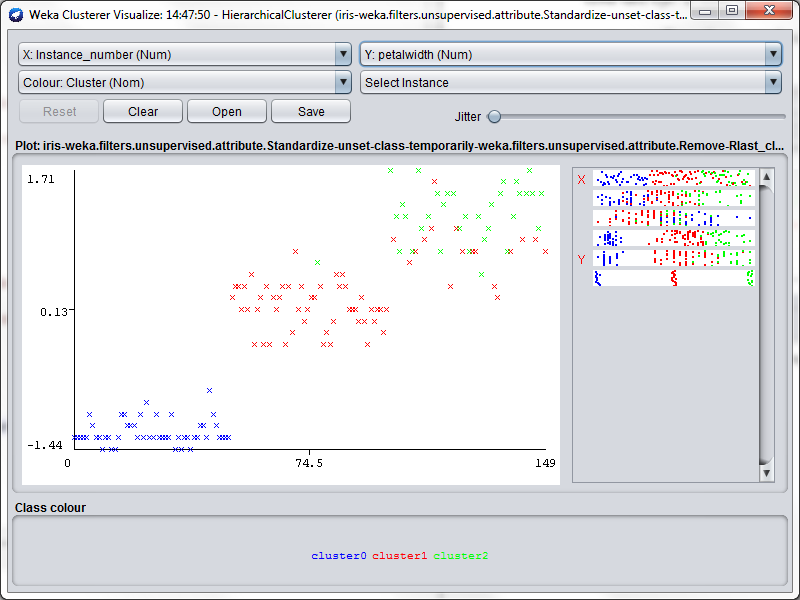
\includegraphics[width=8cm]{hc_petalwidth.png} }}
		\caption{X instance\_number con \textit{petallength} y \textit{petalwidth}.}
		\label{Figura_8}
	\end{figure}
\end{itemize}

En ninguna de ellas, todos los grupos están totalmente diferenciados y con fronteras claras. 

En las gráficas de la Figura \ref{Figura_7} los grupos no se han agrupado correctamente.

En las gráficas de la Figura \ref{Figura_8} los grupos 1 y 2 no se han agrupado correctamente. Sí que se ha agrupado correctamente el grupo 0.

\end{questions}

\end{document}
